%% POUR LE CORRIGÉ : remplacer \corrigefalse par \corrigetrue (dans \begin{document}).
%% Avec \corrigefalse, on obtient le sujet seul (1 page) ; avec \corrigetrue,
%% la même page avec les réponses en rouge.

%% Font size %%
\documentclass[11pt]{article}

%% Load the custom package
\usepackage{Mathdoc}
\usetikzlibrary{calc}
\usepackage{colortbl}

%% Numéro de séquence %% Titre de la séquence %%
\renewcommand{\centerhead}{S04 - Éval : Nature d'un angle}

%% Spacing commands %%
\renewcommand{\baselinestretch}{1} \setlength{\parindent}{0pt}

% Corrigé : la feuille est écrite une seule fois (\feuille).
\newif\ifcorrige
% Réponse (texte) dans une case de largeur fixe : \rep[largeur]{réponse}
\newcommand{\rep}[2][1.6cm]{\makebox[#1]{\ifcorrige\textcolor{red}{\textbf{#2}}\else\dotfill\fi}}
% Mot à entourer : \ent{code}{mot}
%   code 1 = bonne réponse (entourée en rouge dans le corrigé),
%   code 2 = exemple déjà fait (entouré en noir partout), 0 = rien.
\newcommand{\ent}[2]{\def\coulcadre{none}%
  \ifnum#1=1 \ifcorrige\def\coulcadre{red}\fi\fi
  \ifnum#1=2 \def\coulcadre{black}\fi
  \tikz[baseline=(m.base)]\node[draw=\coulcadre,thick,rounded corners=2mm,inner sep=2pt](m){\strut #2};}
% Les quatre natures à entourer : \choixnat[code]{n}  (n = 1 aigu, 2 droit, 3 obtus, 4 plat)
\newcommand{\choixnat}[2][1]{%
  \ent{\ifnum#2=1 #1\else0\fi}{aigu}\hspace{2pt}%
  \ent{\ifnum#2=2 #1\else0\fi}{droit}\hspace{2pt}%
  \ent{\ifnum#2=3 #1\else0\fi}{obtus}\hspace{2pt}%
  \ent{\ifnum#2=4 #1\else0\fi}{plat}}

% Angle de sommet V, de mesure #2 degrés, premier côté orienté à #3 degrés
% (d'après le QCM DS-6C04-05).
% \angleDessin[échelle]{mesure}{rotation}{L1}{V}{L2}
% Si \codedroitfalse : arc pour tous les angles ; dans le corrigé, l'angle
% droit reçoit son petit carré en rouge (non utilisé : angles droits toujours codés).
\newif\ifcodedroit \codedroittrue
\newcommand{\angleDessin}[6][1]{%
  \begin{tikzpicture}[scale=#1]
    \coordinate (V) at (0,0);
    \coordinate (P) at (#3:1.8); \coordinate (Q) at ({#3+#2}:1.8);
    \def\carre{(0,0) -- (#3:3.5mm) -- ($(#3:3.5mm)+({#3+90}:3.5mm)$) -- ({#3+90}:3.5mm) -- cycle}
    \def\arcang{(0,0) -- (#3:4.5mm) arc[start angle=#3, delta angle=#2, radius=4.5mm] -- cycle}
    \ifnum#2=90
      \ifcodedroit \draw[gray!70!black, fill=gray!30] \carre;
      \else\ifcorrige \draw[red, fill=red!20] \carre;
      \else \draw[gray!70!black, fill=gray!30] \arcang;
      \fi\fi
    \else
      \draw[gray!70!black, fill=gray!30] \arcang;
    \fi
    \draw[thick] (P) -- (V) -- (Q);
    \fill (P) circle (0.8pt); \fill (Q) circle (0.8pt); \fill (V) circle (0.8pt);
    \node at (#3:2.1) {$#4$};
    \node at ({#3+#2/2+180}:5mm) {$#5$};
    \node at ({#3+#2}:2.1) {$#6$};
  \end{tikzpicture}%
}

% Une case de l'exercice 1 : \caseangle{mesure}{rotation}{L1}{V}{L2}{n}
\newcommand{\caseangle}[6]{%
  \begin{tabular}{@{}c@{}}
    \angleDessin[0.66]{#1}{#2}{#3}{#4}{#5} \\[-2mm]
    $\widehat{#3#4#5}$ est : \\
    {\small\choixnat{#6}}
  \end{tabular}}
\newcommand{\caseangleex}[6]{%
  \begin{tabular}{@{}c@{}}
    \angleDessin[0.66]{#1}{#2}{#3}{#4}{#5} \\[-2mm]
    \textit{Exemple :} $\widehat{#3#4#5}$ est : \\
    {\small\choixnat[2]{#6}}
  \end{tabular}}

% Vrai / Faux : \vf{1} (vrai) ou \vf{2} (faux)
\newcommand{\vf}[1]{\ent{\ifnum#1=1 1\else0\fi}{Vrai}\,/\,\ent{\ifnum#1=2 1\else0\fi}{Faux}}

\newcommand{\feuille}{%
\phantom{0}
\vspace{-.5cm}

\entetedevoirs{20}

\begin{center}
\duree{20 minutes}
\total{20 points}
\calculatrice{0}
\textit{Les angles droits sont codés par un petit carré.}
\end{center}

\vspace{-0.6cm}
\begin{exercicedevoir}[6][Sur une figure]
\vspace{-0.3cm}
Pour chaque angle, compare-le à l'angle droit, puis \textbf{entoure} sa nature.

\codedroittrue
\renewcommand{\arraystretch}{1}
\begin{tabularx}{\linewidth}{@{}*{4}{>{\centering\arraybackslash}X}@{}}
\caseangleex{145}{10}{A}{B}{C}{3} &
\caseangle{65}{200}{D}{E}{F}{1} &
\caseangle{90}{120}{G}{H}{I}{2} &
\caseangle{180}{30}{J}{K}{L}{4} \\[2mm]
\caseangle{125}{30}{M}{N}{P}{3} &
\caseangle{25}{80}{R}{S}{T}{1} &
\caseangle{90}{345}{U}{V}{W}{2} &
\\
\end{tabularx}
\end{exercicedevoir}

\vspace{-1.1cm}
\begin{exercicedevoir}[6][Avec la mesure]
\vspace{-0.3cm}
Complète avec : \textbf{nul}, \textbf{aigu}, \textbf{droit}, \textbf{obtus} ou \textbf{plat}.

\smallskip
\renewcommand{\arraystretch}{1.45}
\begin{tabularx}{0.97\linewidth}{|l|*{7}{>{\centering\arraybackslash}X|}}
\hline
\textbf{Mesure de l'angle} & \cellcolor{gray!15}$150^\circ$ & $45^\circ$ & $180^\circ$ & $92^\circ$ & $0^\circ$ & $90^\circ$ & $88^\circ$ \\ \hline
\textbf{Nature de l'angle} & \cellcolor{gray!15}\textit{obtus} & \rep[\linewidth]{aigu} & \rep[\linewidth]{plat} & \rep[\linewidth]{obtus} & \rep[\linewidth]{nul} & \rep[\linewidth]{droit} & \rep[\linewidth]{aigu} \\ \hline
\end{tabularx}
\end{exercicedevoir}

\vspace{-1.1cm}
\begin{exercicedevoir}[5][Dans une figure]
\vspace{-0.3cm}
\begin{minipage}[c]{0.35\linewidth}
\centering
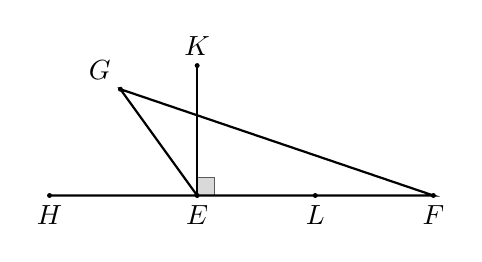
\begin{tikzpicture}[scale=0.75]
  \coordinate (H) at (-2.5,0); \coordinate (E) at (0,0); \coordinate (L) at (2,0);
  \coordinate (F) at (4,0); \coordinate (G) at (-1.3,1.8); \coordinate (K) at (0,2.2);
  \draw[gray!70!black, fill=gray!30] (E) rectangle ++(0.3,0.3);
  \draw[thick] (H) -- (F) -- (G) -- (E); \draw[thick] (E) -- (K);
  \foreach \p in {H,E,L,F,G,K} \fill (\p) circle (1.2pt);
  \node[below] at (H) {$H$}; \node[below] at (E) {$E$}; \node[below] at (L) {$L$};
  \node[below] at (F) {$F$}; \node[above left] at (G) {$G$}; \node[above] at (K) {$K$};
\end{tikzpicture}
\end{minipage}%
\hfill
\begin{minipage}[c]{0.64\linewidth}
Les points $H$, $E$, $L$ et $F$ sont alignés. Complète.

\renewcommand{\arraystretch}{1.5}
\begin{tabular}{@{}ll@{}}
\textit{Exemple :} $\widehat{GEF}$ est un angle obtus. & $\widehat{HEF}$ est un angle \rep[1.4cm]{plat}. \\
$\widehat{EFG}$ est un angle \rep[1.4cm]{aigu}. & $\widehat{KEF}$ est un angle \rep[1.4cm]{droit}. \\
$\widehat{HEG}$ est un angle \rep[1.4cm]{aigu}. & $\widehat{LEF}$ est un angle \rep[1.4cm]{nul}. \\
\end{tabular}
\end{minipage}
\end{exercicedevoir}

\vspace{-1.1cm}
\begin{exercicedevoir}[3][Vrai ou faux ?]
\vspace{-0.3cm}
Entoure la bonne réponse.

\renewcommand{\arraystretch}{1.2}
\begin{tabular}{@{}l@{\qquad}l@{}}
a) Un angle de $150^\circ$ est un angle obtus. & \vf{1} \\
b) Un angle plat mesure $90^\circ$. & \vf{2} \\
c) Un angle aigu peut mesurer $95^\circ$. & \vf{2} \\
\end{tabular}
\end{exercicedevoir}

\vspace{-0.6cm}
{\small\competences{
6C04-GEO12 & Reconnaître la nature d'un angle & & & & \\ \hline
}}
}

\begin{document}

\corrigefalse
\feuille

\end{document}

%%% Local Variables:
%%% mode: LaTeX
%%% TeX-master: t
%%% End:
